% !TEX root = ../main.tex
\chapter{Demonstrationsversuch}
\begin{figure}[tb]
	\begin{subfigure}{.4\textwidth}
		\centering
		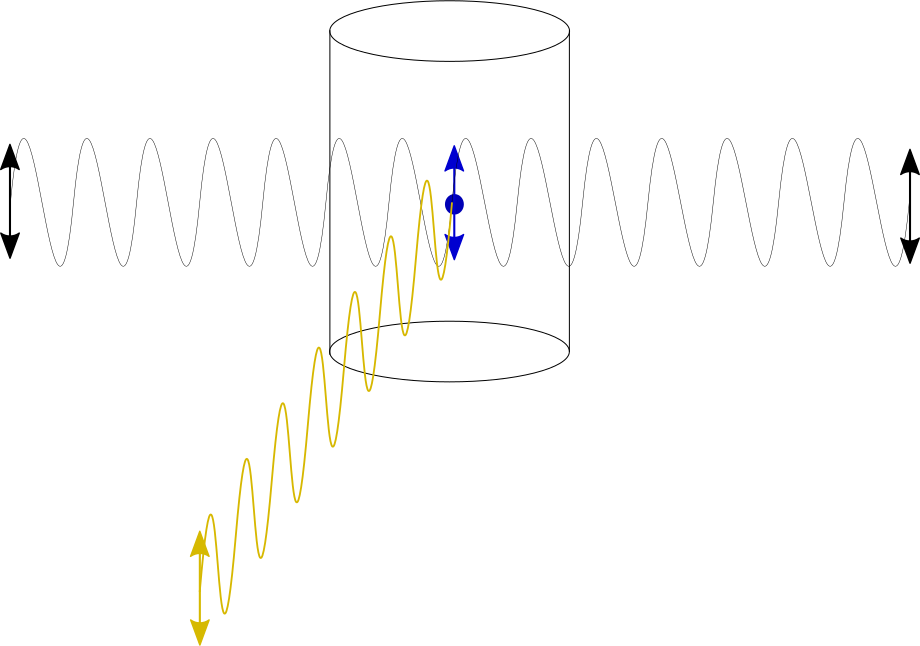
\includegraphics[height=.8\linewidth]{./img/pol_streu_vert.pdf}
		\caption[Vertikale Komponente]{Polarisation durch Streuung: Vertikale Komponente des unpolarisierten Lichtes}
	\end{subfigure}
	$\quad$
	\begin{subfigure}{.4\textwidth}
		\centering
		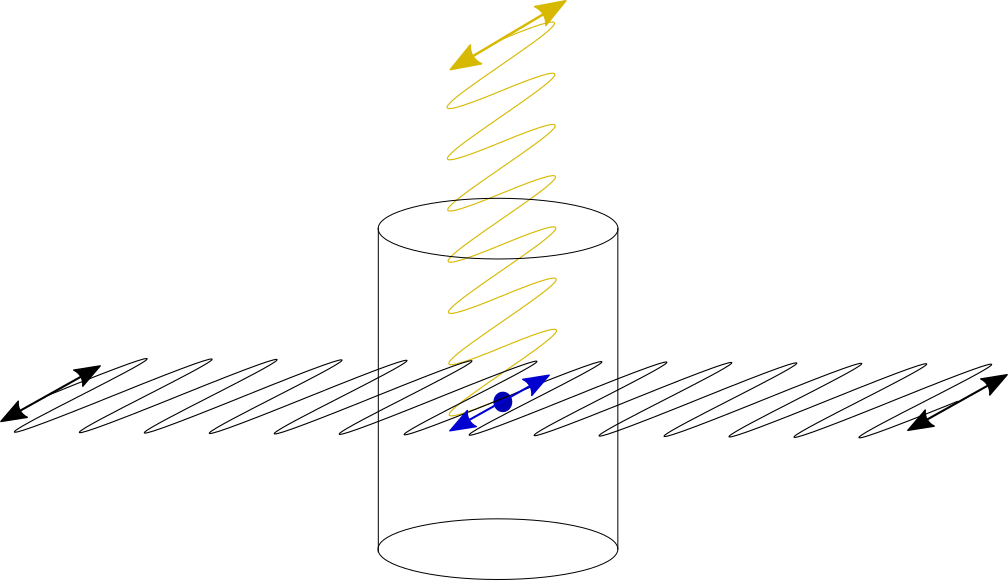
\includegraphics[height=.8\linewidth]{./img/pol_streu_hori.pdf}
		\caption[Horizontale Komponente]{Polarisation durch Streuung: Horizontale Komponente des unpolarisierten Lichtes}
	\end{subfigure}
	\caption[Visualisierung der Richtungsabhängigkeiten]{Abhängigkeit der Dipolstrahlung von der Richtung des einfallenden Lichtes}
	\label{fig:pol_streu}
\end{figure}

Zur Demonstration von Polarisation durch Streuung wird unpolarisiertes Licht auf ein Glas Wasser gerichtet.
Dabei wird das Licht mithilfe einer Blende zu einem Strahl geformt, welcher innerhalb des Wassers aufgrund von Streuung sichtbar ist.
Das am Wasser gestreute Licht wird durch einem Polarisationsfilter von verschiedenen Seiten beobachtet.
Dabei ist zu erkennen, dass das Streulicht aus verschiedenen Richtungen betrachtet unterschiedlich polarisiert ist.
Wird eine feste Streurichtung betrachtet, so kann bei einer Polarisationsrichtung ein Intensitätsmaximum festgestellt werden, während bei einem zu diesem Winkel um \SI{90}{\degree} gedrehten Winkel nahezu kein Licht mehr sichtbar ist.
Daraus ist zu schließen, dass das einfallende unpolarisierte Licht durch die Streuung am Medium Wasser polarisiert wird.

Werden die Wassermoleküle als Oszillatoren aufgefasst, die von dem einfallenden Licht zu Schwingungen angeregt werden, so lässt sich das Phänomen erklären.
Durch das einfallende Licht werden innerhalb der Moleküle Ladungen angeregt, welche ihrerseits eine Dipolstrahlung emittieren.
Diese wird vorzugsweise orthogonal zu ihrer Schwingungsrichtung ausgesendet, jedoch niemals entlang der Dipolachse.
Erwähnte Richtungsbeziehungen werden in \autoref{fig:pol_streu} dargestellt.
Das so auslaufende Licht ist nahezu vollständig polarisiert, weshalb einen Polarisationsfilter nur in der richtigen Ausrichtung passieren kann.
